\subsection*{Partie I. Caractérisation d'un polygone régulier direct.}
\begin{enumerate}
 \item En utilisant le conjugué du dénominateur, on trouve
\begin{align*}
 \frac{1+3i}{1-i}= -1+2i & & \frac{3+i}{1-i}= 1+2i  
\end{align*}
\item
\begin{enumerate}
\item D'après le cours sur l'expression complexe d'une rotation, $r(z)=g+e^{i\alpha}(z-g)$.
\item On compose les $r$ puis on somme:
\begin{multline*}
 \left\lbrace 
\begin{aligned}
 & a_1 = g +1(a_1-g)\\
 &r(a_1) = g + e^{i\alpha}(a_1-g)\\
 &r^2(a_1) = g + e^{i2\alpha}(a_1-g)\\
 &\vdots   \\
 &r^{n-1}(a_1) = g + e^{i(n-1)\alpha}(a_1-g)\\
\end{aligned}
\right. \\
\Rightarrow
a_1+r(a_1)+\cdots+r^{n-1}(a_1) 
= ng + (\underset{=0}{\underbrace{1+e^{i\alpha}+\dots+e^{i(n-1)\alpha}}})(a_1-g)
= ng
\end{multline*}
\end{enumerate}
\item La définition d'un polygone régulier direct comporte $n$ relations. Dans la question a., on considère seulement les $n-1$ premières et dans la question $b$ les $n-2$ premières. Pour chaque question une des implications est donc évidente, on se concentre donc sur la réciproque.
\begin{enumerate}
 \item Les $n-1$ premières relations entrainent $A_k=R^{k-1}(A_1)$ pour $k$ entre $2$ et $n$. On obtient $R(A_n)=R^n(A_1$ en composant la dernière relation par $R$. Or $R^n$ est l'identité par définition de $\alpha$. La dernière relation est donc bien vérifiée.
 \item Cette fois ci, $A_k=R^{k-1}(A_1)$ n'est valable que pour $k$ entre $2$ et $n-1$. Mais, d'après 2.b.
\begin{displaymath}
 a_1 + \underset{=a_2}{r(a_1)}+\cdots+\underset{=a_{n-1}}{r^{n-2}(a_1)}+r^{n-1}(a_1)=ng= a_1+\cdots +a_n
\end{displaymath}
On en tire la relation manquante.
\end{enumerate}
\item D'après 3.b., un triangle équilatéral direct est caractérisé par la seule relation $A_2=R(A_1)$. Elle s'écrit
\begin{multline*}
 a_2-\frac{1}{3}\left(a_1+a_2+a_3 \right) = j\left(a_1- \frac{1}{3}\left(a_1+a_2+a_3 \right)\right)  \\
\Leftrightarrow
(-1-2j)a_1 + (2+j)a_2 + (-1+j)a_3 = 0
\end{multline*}
Elle se simplifie grace à
\begin{align*}
 &-1-2j &= -\sqrt{3}i\\
 &2+j &= \frac{3}{2}+i\frac{\sqrt{3}}{2}= -\sqrt{3}ij\\
 &-1+j &= -\frac{3}{2}+i\frac{\sqrt{3}}{2}= -\sqrt{3}ij^2
\end{align*}
qui permet de simplifier par $-\sqrt{3}i$ et conduit à 
\begin{displaymath}
 a + jb + j^2c =0
\end{displaymath}
\item 
\begin{enumerate}
\item D'après 3.b., un carré direct est caractérisé par les deux relations $A_2=R(A_1)$ $A_3=R(A_2)$. On se concentre sur la première car la deuxième se déduira par permutation des indices. Elle s'écrit
\begin{multline*}
a_2-\frac{1}{4}\left(a_1+a_2+a_3 +a_4\right) = j\left(a_1- \frac{1}{4}\left(a_1+a_2+a_3 +a_4\right)\right)  \\ 
\Leftrightarrow
-a_1+3a_2-a_3-a_4 = i(3a_1-a_2-a_3-a_4) \\
\Leftrightarrow
-(1+3i)a_1+(3+i)a_2+(-1+i)a_3+(-1+i)a_4\\
\Leftrightarrow
\frac{1+3i}{1-i}a_1 - \frac{3+i}{1-i}a_2 + a_3 + a_4 = 0
\end{multline*}
On obtient alors la première des deux relations demandées en utilisant le résultat de la question 1. La seconde relation s'obtient en permutant circulairement les indices.
\item Notons $R_1$ et $R_2$ les deux relations du a.
\begin{multline*}
 R_1 + R_2 
\Leftrightarrow 2ia_1 - 2a_2 -2ia_3 +2a_4 =0 \\
\Leftrightarrow a_1 + ia_2 -a_3-ia_4 \text{ (en divisant par $2i$) }
\Leftrightarrow a_1+ia_2 = a_3 + ia_4
\end{multline*}
\begin{multline*}
 iR_1 + R_2
\Leftrightarrow
(-i-1)a_1 + (i+1)a_2 + (-1-i)a_3 + (1+i)a_4 = 0 \\
\Leftrightarrow a_1 + a_3 = a_2+a_4 \text{ (en divisant par $1+i$) }
\end{multline*}
Il est clair que
\begin{displaymath}
\left\lbrace 
\begin{aligned}
 R_1 \\ R_2
\end{aligned}
\right. 
\Rightarrow
\left\lbrace 
\begin{aligned}
 R_1 + R_2\\ iR_1 +R_2
\end{aligned}
\right. 
\end{displaymath}
Réciproquement,
\begin{displaymath}
\left\lbrace 
\begin{aligned}
 R_1 + R_2\\ iR_1 +R_2
\end{aligned}
\right. 
\Rightarrow
\left\lbrace 
\begin{aligned}
 (R_1 + R_2) -(iR_1 +R_2)&= (1-i)R1\\ -i(R_1 + R_2) +(iR_1 +R_2) &= (1-i)R_2
\end{aligned}
\right. 
\Rightarrow
\left\lbrace 
\begin{aligned}
 R_1 \\ R_2
\end{aligned}
\right. 
\end{displaymath}
Les deux systmes sont donc équivalents.\newline
La première relation traduit l'orthogonalité directe des diagonales et la deuxième le fait qu'elles se coupent en leur milieu.
\end{enumerate}
\end{enumerate}

\subsection*{Partie II. Triangles semblables.}
\begin{enumerate}
 \item Notons $T$ l'expression à transformer. La relation de cours exprimant le carré du module d'une somme de deux complexes s'étend naturellement à trois. En l'utilisant, les carrés des modules se simplifient ce qui conduit à
\begin{displaymath}
 T = 2\Re \left( 
a\bar{b}\bar{j} + a\bar{c}j + b\bar{c}\bar{j} - a\bar{b}j + a\bar{c}\bar{j} + b\bar{c}j   
\right) 
=2\sqrt{3}\Im\left( 
a\bar{b} - a\bar{c} + b\bar{c}
\right) 
\end{displaymath}
car $j-\bar{j}=i\sqrt{3}$ et $\Re(iz)=-\Im(z)$.\newline
Comme de plus, $\Im(a\bar{c})=-\Im(\bar{a\bar{c}}) = -\Im(c\bar{a})$, on obtient finalement
\begin{displaymath}
 T = 2\sqrt{3}\Im\left( a\bar{b} +b\bar{c} + c\bar{a}\right) 
\end{displaymath}

 \item Traduisons l'alignement des points
\begin{multline*}
 A, B, C \text{ alignés} \Leftrightarrow \frac{c-a}{b-a}\in \R
\Leftrightarrow (c-a)(\bar{b}-\bar{a})\in \R \\
\Leftrightarrow c\bar{b} - a\bar{b} -c\bar{a} +|a|^2 \in \R
\Leftrightarrow c\bar{b} - a\bar{b} -c\bar{a} \in \R
\end{multline*}
Or $c\bar{b}+b\bar{c}=2\Re(c\bar{b})$. On peut donc conclure
\begin{displaymath}
 A, B, C \text{ alignés}
 \Leftrightarrow -b\bar{c}+2\Re(c\bar{b}) - a\bar{b} -c\bar{a} \in \R
\Leftrightarrow b\bar{c}+ a\bar{b} +c\bar{a} \in \R
\end{displaymath}

 \item 
\begin{enumerate}
 \item D'après la première partie, $W(A,B,C)$ n'est pas défini lorsque $(A,C,B)$ est un triangle équilatéral direct. On dira alors que $(A,B,C)$ est un triangle équilatéral indirect.
 \item D'après 1. et 2., le complexe $W(A,B,C)$ est de module $1$ si et seulement si $A$, $B$, $C$ sont alignés.
\end{enumerate}

 \item 
\begin{enumerate}
 \item Supposons $(A,B,C)$ et $(A',B',C')$ directement semblables avec
\begin{align*}
 a' = ua+v & & b'=ub+v & & c'=uc+v
\end{align*}
alors:
\begin{displaymath}
 a'+j^2b'+jc' = u(a+j^2b+jc) + (1+j^2+j)v = u(a+j^2b+jc)
\end{displaymath}
De même, $a'+jb'+j^2c' = u(a+jb+j^2c)$. On en déduit que les deux triangles sont simultanément indirectement semblables ou bien qu'ils ont le même $W$.
 \item On suppose $W(A,B,C)$ et $W(A',B',C')$ définis et égaux. On veut montrer qu'il existe des complexes $u\neq 0$ et $v$ tels que
\begin{align*}
 a' = ua+v & & b'=ub+v & & c'=uc+v
\end{align*}
Analyse. S'il existe de tels complexes $u$ et $v$
\begin{displaymath}
 \left\lbrace 
\begin{aligned}
 a' &= ua +v\\b' &= ub+v
\end{aligned}
\right. 
\Rightarrow
 \left\lbrace 
\begin{aligned}
 u &= \frac{b'-a'}{b-a}\\ v &= \frac{ba'-ab'}{b-a}
\end{aligned}
\right. 
\end{displaymath}
 Synthèse. Posons
\begin{displaymath}
 u = \frac{b'-a'}{b-a}, \hspace{0.5cm} v = \frac{ba'-ab'}{b-a}
\end{displaymath}
et vérifions que $a'=ua+v$, $b'=ub+v$, $c'=uc+v$. C'est facile pour les deux premières relation à cause de la définition de $u$ et $v$. Il reste à montrer
\begin{displaymath}
 (E)\hspace{1cm} c' = \frac{b'-a'}{b-a}c + \frac{ba'-ab'}{b-a}
\end{displaymath}
On peut former des relations équivalentes
\begin{displaymath}
 (E)\Leftrightarrow (b-a)c'=(b'-a')c+ba'-ab'
\Leftrightarrow (ab'-a'b) + (bc'-cb') + (ca'-ac') = 0
\end{displaymath}
On peut aussi traduire l'égalité des $W$. Après calculs, on obtient
\begin{multline*}
 (a+jb+j^2c)(a'+j^2b'+jc')-(a'+jb'+j^2c')(a+j^2b+jc) \\
= (j^2-j)\left( (ab'-a'b) + (bc'-cb') + (ca'-ac')\right) 
\end{multline*}
Ce qui montre que l'égalité de $W$ entraine $(E)$.
\end{enumerate}

 \item Les deux expressions $W(A,B,C)$ et $W(A',B',C')$ sont bien définies si et seulement si $(A,B,C)$ n'est pas équilatéral (ni directement, ni indirectement). On trouve alors que
\begin{displaymath}
 W(A',B',C') = \frac{1}{\bar{W(A,B,C)}}
\end{displaymath}
\end{enumerate}

\subsection*{Partie III. Construction.}
\begin{enumerate}
 \item 
\begin{enumerate}
 \item On construit $A_1$ en remarquant que $\overrightarrow{AA_1}$ est l'image de $\overrightarrow{BC}$ par la rotation vectorielle d'angle $\frac{\pi}{2}$. De même pour les autres points.
 \item En sommant les définitions, les termes en $i$ se simplifient
\begin{displaymath}
 \left. 
\begin{aligned}
 a_1 &= a +ib -ic \\ b_1 &= -ia +b +ic \\ c_1 &= ia -ib +c 
\end{aligned}
\right\rbrace 
\Rightarrow
a_1+b_1+c_1 = a+b+c
\end{displaymath}
Les deux triangles ont donc le même centre de gravité.
 \item Le triangle $(A_1,B_1,C)$ est rectangle et isocèle en $C$ car
\begin{displaymath}
 a_1-c = a-c +i(b-c) = i\left( b-c +i(c-a)\right) = i(b_1-c) 
\end{displaymath}
De même pour les autres par permutation circulaire.
\end{enumerate}

 \item 
\begin{enumerate}
 \item Formons les équations traduisant les conditions
\begin{displaymath}
 \left\lbrace 
\begin{aligned}
 a+ib-ic &= 1 \\ -ia+b+ic &= -1 \\ ia -ib +c &= x
\end{aligned}
\right. 
\end{displaymath}
En ajoutant les deux premières, on tire
\begin{displaymath}
 (1-i)a+(1+i)b=0 \Rightarrow b = ia
\end{displaymath}
En injectant dans la deuxième, on déduit $c=i$. La troisième permet alors d'exprimer $a$
\begin{displaymath}
 ia+a+i = x \Rightarrow a =\frac{x-i}{1+i}=\frac{x-1-(x+1)i}{2}
\end{displaymath}
 \item Le point $A$ décrit la droite passant par le point de coordonnées $(-\frac{1}{2},-\frac{1}{2})$ et dirigée par le vecteur de coordonnées $(1,-1)$. Le point $B$ décrit la droite obtenue à partir de la précédente par une rotation d'angle $\frac{\pi}{2}$ et de centre l'origine.
\end{enumerate}
\begin{figure}[h!]
 \centering
 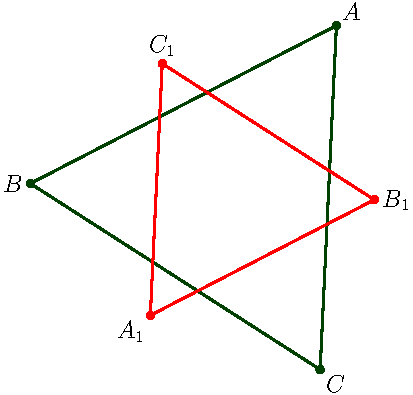
\includegraphics{./Ccomp12_1.pdf}
 % Ccomp12_1.pdf: 198x187 pixel, 72dpi, 6.99x6.60 cm, bb=0 0 198 187
 \caption{Triangles $(A,B,C)$ et $(A_1,B_1,C_1)$ semblables}
 \label{fig:Ccomp12_1}
\end{figure}

 \item Dans cette question, on étudie l'éventualité que les triangles $(A,B,C)$ et $(A_1,B_1,C_1)$ soient directement semblables.
\begin{enumerate}
 \item On trouve
\begin{align*}
 1-ij+ij^2 = 1+\sqrt{3}, & &
 i+j-ij^2 = (1+\sqrt{3})j, & &
 -i+ij+j^2 = (1+\sqrt{3})j^2
\end{align*}

 \item D'après la question a.
\begin{displaymath}
 a_1+jb_1+j^2c_1 = (1+\sqrt{3})(a+jb+j^2c)
\end{displaymath}

 \item De même après calculs, on trouve
\begin{displaymath}
 a_1+j^2b_1+jc_1 = (1-\sqrt{3})(a+j^2b+jc)
\end{displaymath}

 \item D'après les formules précédentes, les triangles $(A,B,C)$ et $(A_1,B_1,C_1)$ ne peuvent avoir le même $W$ que si celui ci est nul ou non défini c'est à dire pour $(A,B,C)$ équilatéral.
 \item  Si $(A,B,C)$ est équilatéral direct alors $W(A,B,C)=W(A',B',C')=0$ et les deux triangles sont directement semblables. Ils ont le même $W$ et ils sont tous les deux directement équilatéraux.\newline
Le centre de la similitude est forcément le centre de gravité commun aux deux triangles. Si la similitude faisant passer d'un triangle à l'autre est de la forme $z\rightarrow uz+v$, le rapport de cette similitude est le module de $u$ et son angle est un argument de $u$.\newline
On a vu en partie II une expression de $u$:
\begin{displaymath}
 u = \frac{b_1-a_1}{b-a}=\frac{b-a + i(2c-a-b)}{b-a}
\end{displaymath}
Introduisons le centre de gravité $g$. Le caractère équilatéral direct de $(A,B,C)$ se traduit par $b-g = j(a-g)$ et $c-g=j^2(a-g)$. On en tire
\begin{displaymath}
 u= \frac{b-a + i(3c-a-b-c)}{b-a}= 1 +3i\frac{c-g}{b-g+ga}=1+3i\frac{j^2}{j-1}=1-\sqrt{3}
\end{displaymath}
après calculs. Comme il s'agit d'un nombre réel strictement négatif,  le rapport est $\sqrt{3}-1$ et l'angle $\pi$. Ces résultats sont bien cohérents avec la figure \ref{fig:Ccomp12_1}.
\end{enumerate}

\end{enumerate}
